\chapter{Novel Work}

In this section the work completed so far will be presented. Two main areas of the systematic review process has been focused on. Stopping criteria and indexing/querying pubmed.

\section{Random Sample Method to Stopping}

As approach to determining when to stop looking at document abstracts returned by the query we are proposing a new sampling method. This approach assumes we have optimum ranking algorithm for returning documents for a query.

The first step of this method is to randomly sample a returned set of documents into a subsets. 

\begin{equation}
U = \frac{|D|}{S}
\end{equation}

Where $U$ is the computed randomised subset, $D$ is the document collection and $S$ is the sample size.

We then use this subset $U$ to create a model / baseline for our topic as a way of predicting how many documents one would need to look at to hit a threshold. The intuition behind this approach is that the rate of which relevant documents occur should be relatively similar when the number of returned documents in the same.

A limitation of this sampling method is that for topics with very few documents it is easy for a sample to miss many of them. This creates a subset set bias, where one set contains a larger percentage of relevant documents. Consider a query that returns 10000 candidate documents of which only 10 have been pre-determined to be relevant. Its not too unlikely that a randomly sampled subset would contain 0 relevant documents. We can use the following equation to tell us how much information we can take from a pre-evaluated topic:

\begin{equation}
I = \frac{rel(T_i)}{|T_i|}
\end{equation}

Where $T_i$ is a given topic and $rel$ computes the number of relevant documents for that topic. Therefore $I$ is telling us how useful the topic is at fitting a curve. We can take the average simply by taking the mean of $I$ across all topics:

\begin{equation}
Usefullness = \frac{\sum{I}}{|T|}
\end{equation}



\subsection{Curve Fitting}

Our first approach uses a simple curve fit against a sample set along with a simple non-linear function. $f(x)$

\begin{equation}
F(x) = n - a\exp^{-kx}
\end{equation}

Where $a$, $k$ and $n$ are learnt weights and $x$ is an associated return rate for a document.

We can visualise the curve along with the confidence intervals. The Y axis is the predicted number of relevant documents for the topic. X axis shows the true number of documents returned for the query. 

\begin{figure}[H]
\center
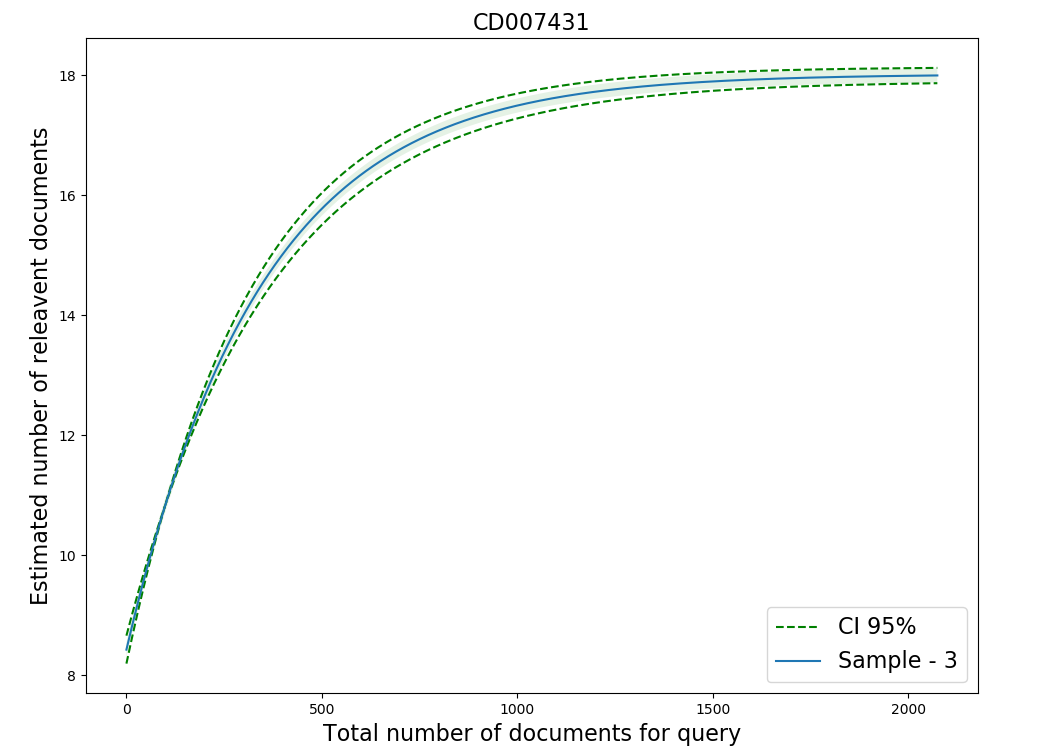
\includegraphics[width=10cm]{figures/curve_fit_example.png}
\caption{Example of fitting a curve for a topic using sampling}
\end{figure}

\begin{table}[H]
\centering
\begin{tabular}{|c|c|c|c|} 

 \hline
 sample size & recall & reliability & effort  \\ 
 1 & 0.91 &	0.96	&	1 \\ 
 3 & 0.66 & 0.5	&	0.48 \\ 
 5 & 0.481 & 0.33	&	0.315 \\ 
 \hline
\end{tabular}
\caption{Comparison of different sample sizes against recall and effort. Ranking Method: Test\_Data\_Sheffield-run-2 \cite{Alharbi2017}}

\end{table}

The first sample size of 1 is included to show how the effort metric is effected. For us to use sample everything, we would need to look at everything, as such the effort averaged out at 1. In this example we were only concerned in achieving 70\% recall, as such even when sampling everything we would really obtain 100\% recall at the expense of 100\% effort.

Looking at every 3rd document and then producing a prediction curve will reduce our effort. We are still required to look at at 1/3 of documents, as such the effort will always be above 0.33. 

\subsubsection{Relevance Ranking}

Our results so far have been based on Test\_Data\_Sheffield-run-2 \cite{Alharbi2017} of CLEF 2017. Naturally, the reliability of our curve is heavily based on how good the initial rankings are for each topic. We can compare different ranking methods for generating our stopping curve. By looking at the CLEF 2017 technology assisted review task \cite{Kanoulas12017} we can determine the best candidates to use.

We also introduce a new field. Topics sampled is the number of topics that were evaluated using the curve. This is included as some of the ranking methods do not produce enough relevant documents to generate a suitable curve. 

\begin{table}[H]
\centering
\begin{tabular}{|c|c|c|c|c|} 

 \hline
 Submission & recall & reliability & effort & topics sampled  \\ 
 Test\_Data\_Sheffield-run-2 & 0.66 &	0.5	&	0.48 & 30 \\ 
 Waterloo A-rank-cost & 0.65 & 0.41	&	0.39 & 29 \\ 
 Waterloo B-rank-cost & 0.70 & 0.46	&	0.40 & 30 \\ 
 auth run-1 & 0.71 & 0.5	&	0.41 & 30 \\ 
 auth run-2 & 0.67 & 0.46	&	0.40 & 30 \\ 
 ntu run-1 & 0.56 & 0.18	&	0.54 & 22 \\ 
 ucl full-text & 0.55 & 0.36	&	0.70 & 11 \\ 
 \hline
\end{tabular}
\caption{Comparison of different of sample method using curve fitting for different CLEF 2017 runs. Sample size = 3. Results are taken as averages over all topics for search method. No topic drop-out}

\end{table}


This second set of results will use a mandatory drop out parameter for topics with less than 0.5\% of relevant documents.  The maximum number of topics for this dataset remains at 30.

We also include a confidence interval evaluation for lower bounded range of a 90\% confidence interval. The key advantages of using a curve as  method of evaluating stopping criteria is being able to make use of this confidence interval in a real systematic review. In the context of a systematic reviewers at the data filtering stage, we could specify that the system is 90\% certain that 70\% of relevant documents have been found. At which point the reviewer can decide if its worth continuing to look at documents.

\begin{table}[H]
\scalebox{0.8}{
\centering
\begin{tabular}{|c|c|c|c|c|} 

 \hline
 Submission & recall-lower-upper & reliability-lower-upper & effort-lower-upper & topics sampled  \\ 
 Test\_Data\_Sheffield-run-2 & 0.71 \, 0.67 \, 0.71, &	0.57 \, 0.53 \, 0.57	&	0.50 \, 0.48 \, 0.50 & 26 \\ 
 Waterloo A-rank-cost & 0.68 \, 0.67 \, 0.68, &	0.41 \, 0.33 \, 0.41	&	0.40 \, 0.40 \, 0.41 & 24 \\ 
 Waterloo B-rank-cost & 0.72 \, 0.71 \, 0.73, &	0.53 \, 0.53 \, 0.61	&	0.41 \, 0.41 \, 0.41 & 26 \\ 
 auth run-1 & 0.73 \, 0.73 \, 0.74, &	0.52 \, 0.52 \, 0.60	&	0.42 \, 0.42 \, 0.43 & 23 \\ 
 auth run-2 & 0.72 \, 0.72 \, 0.72, &	0.54 \, 0.52 \, 0.54	&	0.42 \, 0.42 \, 0.42 & 22 \\ 
 ntu run-1 & 0.61 \, 0.55 \, 0.60, &	0.26\, 0.25 \, 0.26	&	0.54 \, 0.52 \, 0.54 & 15 \\ 
 ucl full-text & 0.61 \, 0.29 \, 0.58, &	0.5 \, 0.125 \, 0.375	&	0.75 \, 0.52 \, 0.68 & 8 \\ 
 \hline
\end{tabular}
}
\caption{Comparison of different of sample method using curve fitting for different CLEF 2017 runs. Sample size = 3. Results are taken as averages over all topics for search method. with 0.5\% drop-out}

\end{table}

We have deliberately compared two of the better participant rankings (Waterloo and auth) and two of the lower performers (ntu and ucl). We can see the quality of the initial rankings significantly influences the performance of our stopping criteria. This suggests there is a important relationship between using a curve to predict a stopping point and how good the initial ranking of documents is. Some of the ranking methods struggle to produce curves and when combined with a drop-out parameter produce become not worth considering in our evaluation.

\subsection{Gaussian Process fitting}

As an alternate approach to fitting a simple curve, we can apply a GP.

We will apply a constant kernel plus a squared-exponential kernel.

\begin{table}[H]
\centering
\begin{tabular}{|c|c|c|c|c|} 

 \hline
 Submission & recall & reliability & effort & topics sampled [Max 30]  \\ 
 Test\_Data\_Sheffield-run-2 & 0.694 &	0.66	&	0.49 & 30 \\ 

 \hline
\end{tabular}
\caption{Comparison of different of sample method using GP fitting for different CLEF 2017 runs. Sample size = 3. Results are taken as averages over all topics for search method.}

\end{table}

\section{Indexing and Querying Medline using Systematic Review Protocols}

Being able to produce an efficient index of Medline is something highly desirable in the field of medicial research. A more efficient index will produce more concise results when given a query. This could potentially save time in filtering through many non-relevant studies and providing a more concise data-set for reviewers to observe. 

\subsection{Acquiring Key Information from A Systematic Review Protocol}

A systematic review protocol is created before the systematic review process is started. A systematic review protocol describes the rationale, hypothesis, and planned methods of the review. The Medline query is created manually with the help of the protocol. Here we are looking to generate a suitable query/relevant information from the protocol to then automatically query Medline.

We will use RAKE \cite{rake} to extraction key-words from a protocol, which we can see an example of below:

\begin{tcolorbox}

Topic: CD008122 

Title: Rapid diagnostic tests for diagnosing uncomplicated P. falciparum malaria in endemic countries 

Objective: To assess the diagnostic accuracy of RDTs for detecting clinical P. falciparum malaria (symptoms suggestive of malaria plus P. falciparum parasitaemia detectable by microscopy) in persons living in malaria endemic areas who present to ambulatory healthcare facilities with symptoms of malaria, and to identify which types and brands of commercial test best detect clinical P. falciparum malaria.

\end{tcolorbox}

 
\begin{tcolorbox}

endemic countries objective|ambulatory healthcare facilities|rapid diagnostic tests|falciparum parasitaemia detectable|malaria endemic areas|diagnostic accuracy|falciparum malaria

\end{tcolorbox}

The | symbol represents a separation between a phrase. The protcols are pre-processed as follows: Reference removal, lowercase, words less than $N$ length removed, pubmed stoplist. We decided to not perform any stemming/additional manipulation at this stage, due to uncertainty of query format.


